\documentclass{beamer}
\usepackage[utf8]{inputenc}

\usetheme{Madrid}
\usecolortheme{default}
\usepackage{amsmath,amssymb,amsfonts,amsthm}
\usepackage{txfonts}
\usepackage{tkz-euclide}
\usepackage{listings}
\usepackage{adjustbox}
\usepackage{array}
\usepackage{tabularx}
\usepackage{gvv}
\usepackage{lmodern}
\usepackage{circuitikz}
\usepackage{tikz}
\usepackage{graphicx}
\usepackage{multicol}

\setbeamertemplate{page number in head/foot}[totalframenumber]

\usepackage{tcolorbox}
\tcbuselibrary{minted,breakable,xparse,skins}

\definecolor{bg}{gray}{0.95}
\DeclareTCBListing{mintedbox}{O{}m!O{}}{%
  breakable=true,
  listing engine=minted,
  listing only,
  minted language=#2,
  minted style=default,
  minted options={%
    linenos,
    gobble=0,
    breaklines=true,
    breakafter=,,
    fontsize=\small,
    numbersep=8pt,
    #1},
  boxsep=0pt,
  left skip=0pt,
  right skip=0pt,
  left=25pt,
  right=0pt,
  top=3pt,
  bottom=3pt,
  arc=5pt,
  leftrule=0pt,
  rightrule=0pt,
  bottomrule=2pt,
  toprule=2pt,
  colback=bg,
  colframe=orange!70,
  enhanced,
  overlay={%
    \begin{tcbclipinterior}
    \fill[orange!20!white] (frame.south west) rectangle ([xshift=20pt]frame.north west);
    \end{tcbclipinterior}},
  #3,
}
\lstset{
    language=C,
    basicstyle=\ttfamily\small,
    keywordstyle=\color{blue},
    stringstyle=\color{orange},
    commentstyle=\color{green!60!black},
    numbers=left,
    numberstyle=\tiny\color{gray},
    breaklines=true,
    showstringspaces=false,
}

\numberwithin{equation}{section}
\lstset{
  language=Python,
  basicstyle=\ttfamily\small,
  keywordstyle=\color{blue},
  stringstyle=\color{orange},
  numbers=left,
  numberstyle=\tiny\color{gray},
  breaklines=true,
  showstringspaces=false
}


\title{Problem 4.8.26}
\author{Sarvesh Tamgade}

\date{\today} 
\begin{document}

\begin{frame}
\titlepage
\end{frame}

\section{Question}
\begin{frame}{Question}
\textbf{Question}:
Find the coordinates of the foot of the perpendicular drawn from the point
\[
\vec{P} = \myvec{2 \\ -3 \\ 4}
\]
to the \(Y\)-axis.
\end{frame}

\section{Solution}
\begin{frame}[fragile]
    \frametitle{Solution}
he \(Y\)-axis has the direction vector
\[
\vec{e_{2}} = \myvec{0 \\ 1 \\ 0}
\]
and passes through the origin. Its general point is
\[
\vec{Q} = \myvec{0 \\ q \\ 0}.
\]
Any point \(\vec{Q}\) on the \(Y\)-axis satisfies \(x = 0\) and \(z = 0\).

Let \(\vec{P} = \myvec{2 \\ -3 \\ 4}\).

The foot of the perpendicular \(\vec{Q}\) is given by projecting \(\vec{P}\) onto the \(Y\)-axis as
\[
\vec{Q} = \left(\vec{e_{2}}^\top \vec{P}\right) \frac{\vec{e_{2}}}{\|\vec{e_{2}}\|^2}.
\]
\end{frame}
\begin{frame}[fragile]
    \frametitle{Solution}


\[
\vec{e_{2}}^\top \vec{P} = \myvec{0 & 1 & 0} \myvec{2 \\ -3 \\ 4}.
\]

Since 
\[
\|\vec{e_{2}}\|^2 = 0^2 + 1^2 + 0^2 = 1,
\]
the foot of the perpendicular is
\[
\vec{Q} = \left( \myvec{0 & 1 & 0} \myvec{2 \\ -3 \\ 4} \right) \vec{e_{2}}.
\]

\[
\vec{Q} = (-3) \vec{e_{2}} = \myvec{0 \\ -3 \\ 0}.
\]

\end{frame}

\begin{frame}[fragile]
    \frametitle{Solution}

\textbf{Final Answer:} The coordinates of the foot of the perpendicular are
\[
{\myvec{0 \\ -3 \\ 0}}.
\]


\end{frame}
\section{Graph}
\begin{frame}
    \frametitle{Graph}
    \begin{figure}[htbp]
    \centering
    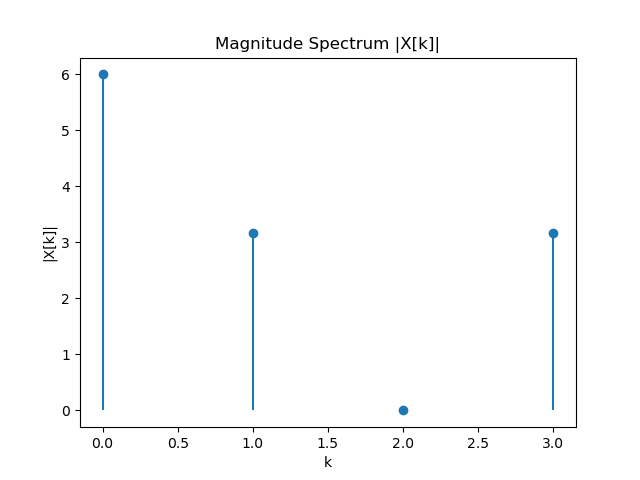
\includegraphics[width=0.65\linewidth]{FIG/fig1.png}
    \caption{Vector Representation}
    \label{fig:FIG/fig1.png}
\end{figure}
\end{frame}
\section{ C Code}
\begin{frame}[fragile]
\frametitle{C Code }
\begin{lstlisting}[language=C]
#include <stdio.h>
#include "matfun.h"

int main() {
    double P[3] = {2.0, -3.0, 4.0};
    double Q[3];

    foot_of_perpendicular_to_Y_axis(P, Q);

    printf("Foot of the perpendicular from P(2, -3, 4) to Y-axis is: (%.2f, %.2f, %.2f)\n", Q[0], Q[1], Q[2]);
    return 0;
}




    
\end{lstlisting}
\end{frame}


\begin{frame}[fragile]
\frametitle{Python Code for Plotting}
\begin{lstlisting}[language=Python]
import matplotlib.pyplot as plt
from mpl_toolkits.mplot3d import Axes3D
import numpy as np

# Points
P = np.array([2, -3, 4])  # Given point
Q = np.array([0, -3, 0])  # Foot of the perpendicular on Y axis

# Y-axis vector for reference
y_axis = np.array([[0, 0], [min(P[1], Q[1]) - 1, max(P[1], Q[1]) + 1], [0, 0]])

fig = plt.figure()
ax = fig.add_subplot(111, projection='3d')

# Plot point P
ax.scatter(P[0], P[1], P[2], color='r', s=100, label='Point P (2, -3, 4)')

\end{lstlisting}

\end{frame}
\begin{frame}[fragile]
\frametitle{Python Code for Plotting}
\begin{lstlisting}[language=Python]
# Plot foot of perpendicular Q
ax.scatter(Q[0], Q[1], Q[2], color='g', s=100, label='Foot of perpendicular Q')

# Plot the perpendicular line from P to Q
ax.plot([P[0], Q[0]], [P[1], Q[1]], [P[2], Q[2]], color='b', label='Perpendicular')

# Plot Y axis
ax.plot(y_axis[0], y_axis[1], y_axis[2], color='k', linestyle='--', label='Y axis')

# Labels and title
ax.set_xlabel('X')
ax.set_ylabel('Y')
ax.set_zlabel('Z')
ax.set_title('Foot of Perpendicular from P to Y axis')

ax.legend()

# Adjust view angle
ax.view_init(elev=20, azim=45)

# Save the figure as .png
plt.savefig('foot_of_perpendicular.png')
plt.show()


\end{lstlisting}

\end{frame}
\begin{frame}[fragile]
\frametitle{Python Code for Plotting}
\begin{lstlisting}[language=Python]
# Adjust view angle
ax.view_init(elev=20, azim=45)

# Save the figure as .png
plt.savefig('foot_of_perpendicular.png')
plt.show()

\end{lstlisting}

\end{frame}
\begin{frame}[fragile]
    \frametitle{Python Code - Using Shared Object}
    \begin{lstlisting}
import ctypes
import numpy as np
import matplotlib.pyplot as plt
from mpl_toolkits.mplot3d import Axes3D

# Load the shared library
matfun_lib = ctypes.CDLL("./matfun.so")

# Define argument types for the C function
# void foot_of_perpendicular_to_Y_axis(const double P[3], double Q[3])
matfun_lib.foot_of_perpendicular_to_Y_axis.argtypes = [
    np.ctypeslib.ndpointer(dtype=np.double, ndim=1, flags="C_CONTIGUOUS"),
    np.ctypeslib.ndpointer(dtype=np.double, ndim=1, flags="C_CONTIGUOUS")
]

\end{lstlisting}
\end{frame}

\begin{frame}[fragile]
    \frametitle{Python Code - Using Shared Object}
    \begin{lstlisting}
# Input point P
P = np.array([2.0, -3.0, 4.0], dtype=np.double)
Q = np.zeros(3, dtype=np.double)  # Output array

# Call the C function to compute the foot of perpendicular
matfun_lib.foot_of_perpendicular_to_Y_axis(P, Q)

# Y-axis vector for plotting
y_axis = np.array([[0, 0], [min(P[1], Q[1]) - 1, max(P[1], Q[1]) + 1], [0, 0]])

# Plotting
fig = plt.figure()
ax = fig.add_subplot(111, projection='3d')

\end{lstlisting}
\end{frame}
\begin{frame}[fragile]
    \frametitle{Python Code - Using Shared Object}
    \begin{lstlisting}
ax.scatter(P[0], P[1], P[2], color='r', s=100, label='Point P (2, -3, 4)')
ax.scatter(Q[0], Q[1], Q[2], color='g', s=100, label='Foot of perpendicular Q')
ax.plot([P[0], Q[0]], [P[1], Q[1]], [P[2], Q[2]], color='b', label='Perpendicular')
ax.plot(y_axis[0], y_axis[1], y_axis[2], color='k', linestyle='--', label='Y axis')

ax.set_xlabel('X')
ax.set_ylabel('Y')
ax.set_zlabel('Z')
ax.set_title('Foot of Perpendicular from P to Y axis')
ax.legend()
ax.view_init(elev=20, azim=45)

plt.savefig('foot_of_perpendicular_from_c.png')
plt.show()


\end{lstlisting}
\end{frame}


\begin{frame}{Plot-Using Both C and Python}
    \centering
    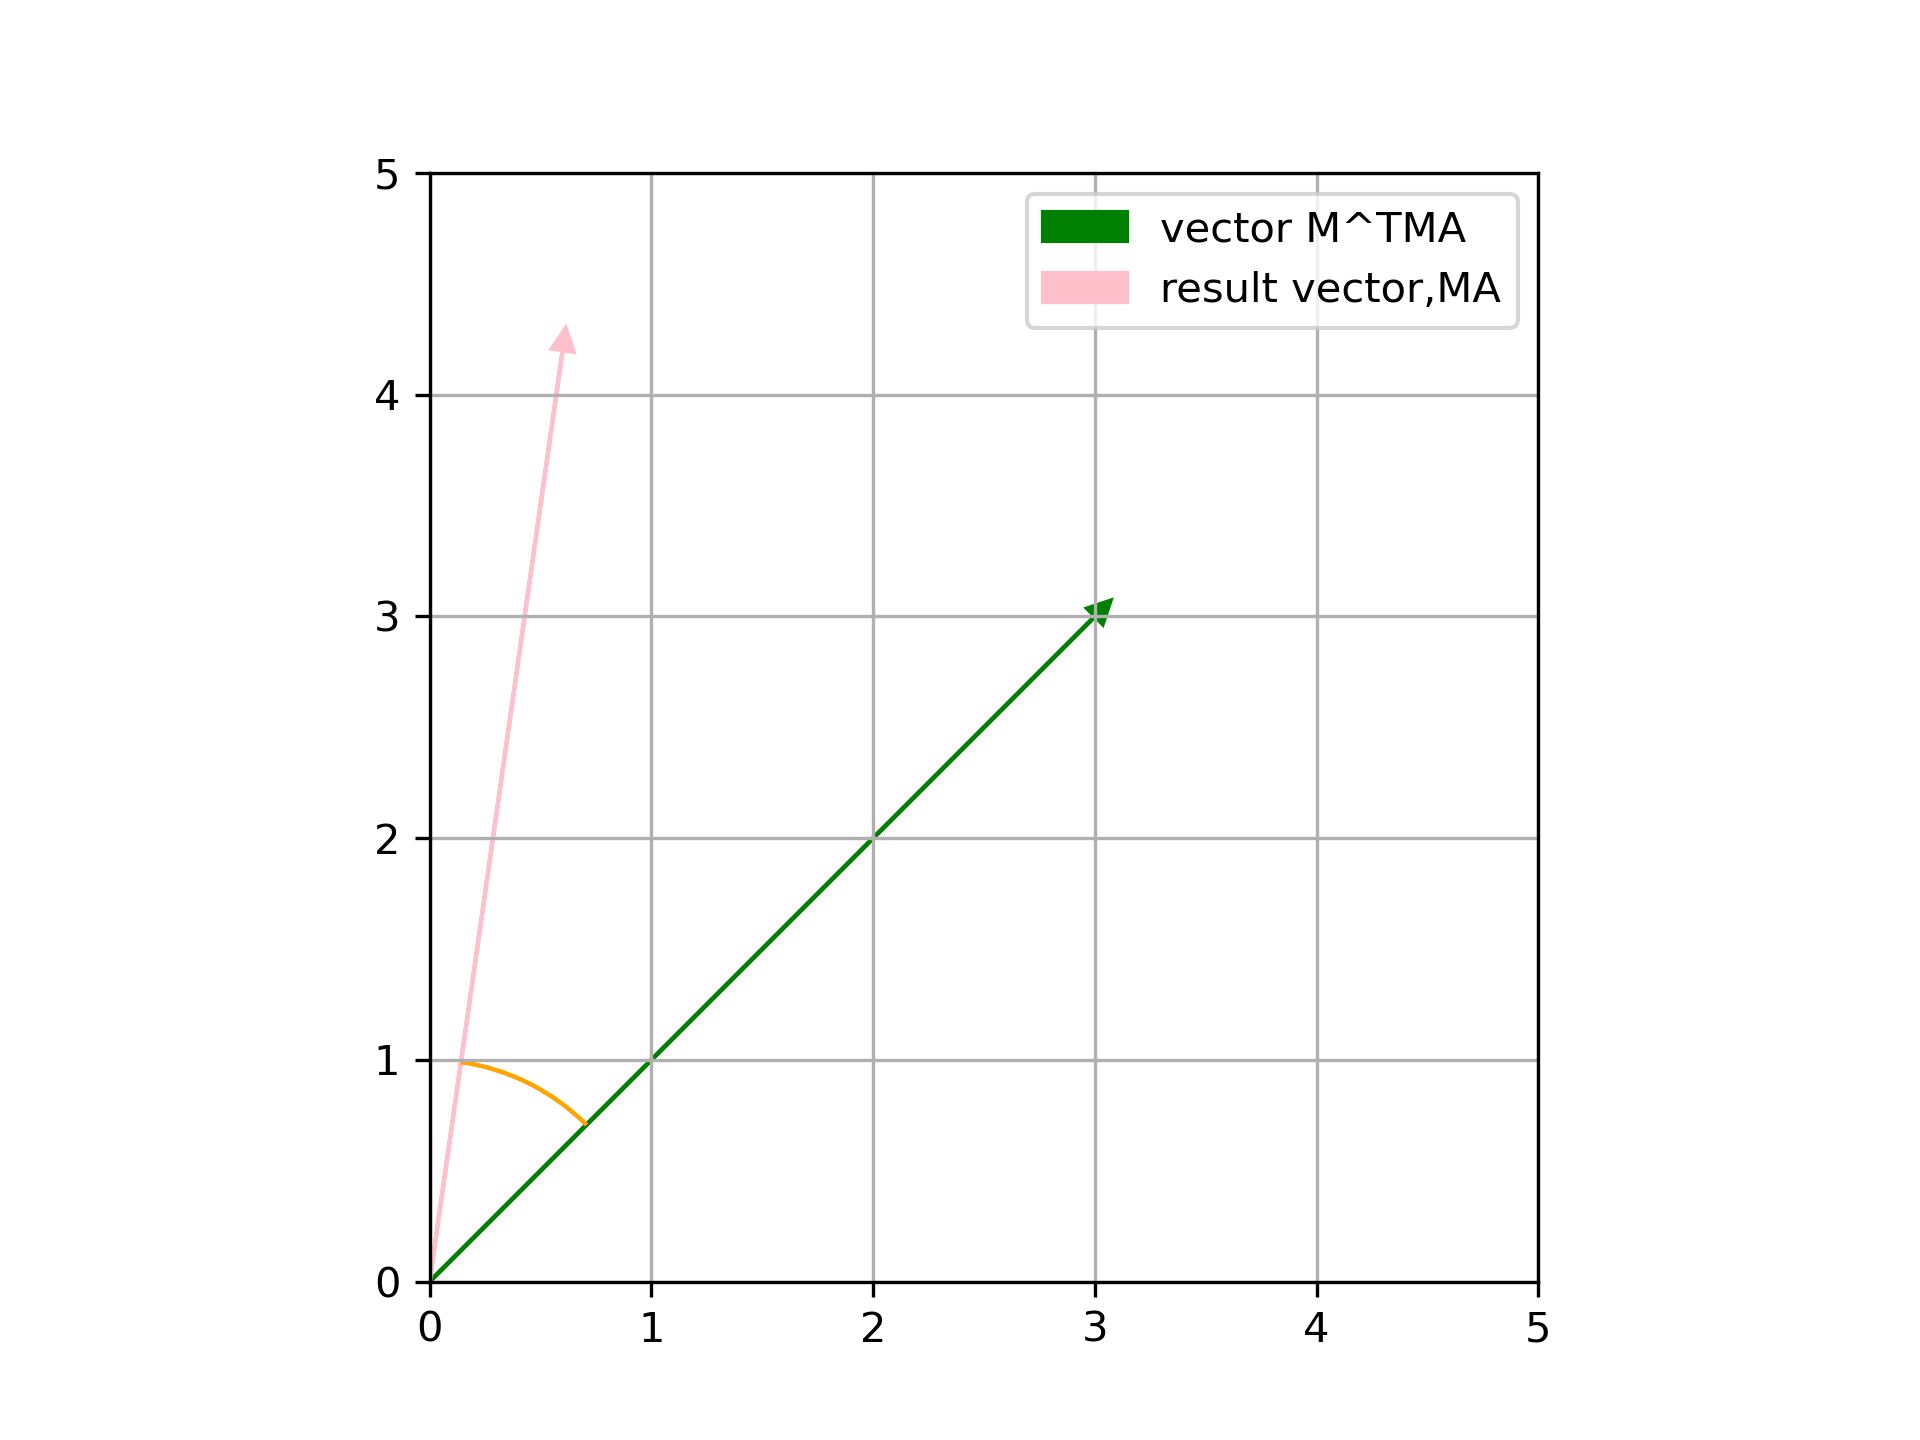
\includegraphics[width=\columnwidth, height=0.8\textheight, keepaspectratio]{FIG/fig2.png}     
\end{frame}


\end{document}
